\documentclass{beamer}
\usetheme{CambridgeUS}
\usepackage{tikz}
\usepackage{listings}
\usepackage{xcolor}

\title{Interrupts}
\subtitle{Embedded Systems}
\author{Group II}
\institute{}
\date{}

\lstset{
    basicstyle=\ttfamily\small,
    keywordstyle=\color{blue},
    commentstyle=\color{green!60!black},
    stringstyle=\color{red},
    breaklines=true
}

\begin{document}

%------------------------------------------------
\frame{\titlepage}

%------------------------------------------------
\begin{frame}{Group Members}
Raymond NTUMWA (S24B23/101) \\
Faith AINOMUGISHA (S24B23/087) \\
Isaac RUBANGANGEYO (S24B23/061) \\
Nathaniel MUGENYI (M24B23/027) \\
Abubaker SSENDAGIRE (S24B23/012)
\end{frame}

%------------------------------------------------
\begin{frame}{What is an Interrupt?}
An interrupt is a signal that makes the microcontroller pause its current task and quickly execute a special function called an Interrupt Service Routine (ISR), before returning to what it was doing.

\vspace{0.5cm}

\textbf{Analogy:} Someone taps your shoulder while reading → you stop → respond → continue reading.
\end{frame}

%------------------------------------------------
\begin{frame}{Why Interrupts Are Important}
Embedded systems handle real-time events:
\begin{itemize}
    \item Button presses
    \item Timer overflows
    \item Sensor triggers
    \item Communication (UART, SPI, I2C)
    \item Motor feedback
\end{itemize}

Without interrupts → Polling wastes CPU time.

\textbf{Interrupts make systems:}
\begin{itemize}
    \item Fast
    \item Efficient
    \item Real-time
    \item Low-power
\end{itemize}
\end{frame}

%------------------------------------------------
\begin{frame}{Types of Interrupts}
\textbf{A. Hardware Interrupts}
\begin{itemize}
    \item Button press
    \item Timer overflow
    \item ADC conversion complete
    \item UART receive complete
\end{itemize}

\textbf{B. Software Interrupts}
\begin{itemize}
    \item System calls
    \item Context switching (RTOS)
    \item Firmware-triggered events
\end{itemize}
\end{frame}

%------------------------------------------------
\begin{frame}{Interrupt Flow Diagram}

\begin{center}
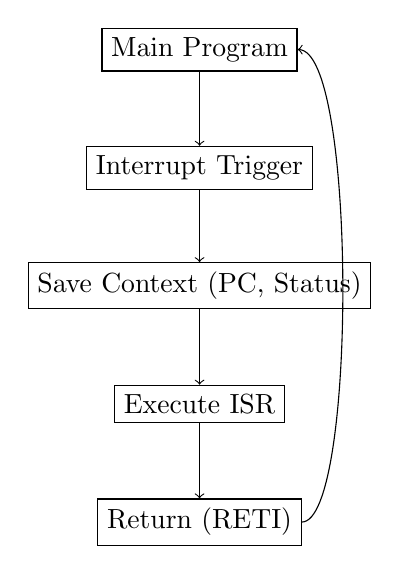
\begin{tikzpicture}[node distance=1.5cm, every node/.style={draw, align=center}]
\node (main) {Main Program};
\node (trigger) [below of=main] {Interrupt Trigger};
\node (save) [below of=trigger] {Save Context (PC, Status)};
\node (isr) [below of=save] {Execute ISR};
\node (return) [below of=isr] {Return (RETI)};

\draw[->] (main) -- (trigger);
\draw[->] (trigger) -- (save);
\draw[->] (save) -- (isr);
\draw[->] (isr) -- (return);
\draw[->] (return) .. controls +(2,0) and +(2,0) .. (main);
\end{tikzpicture}
\end{center}

\end{frame}

%------------------------------------------------
\begin{frame}{How a Timer Interrupt Works}

\begin{center}
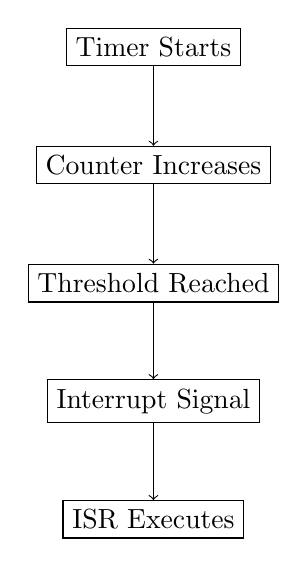
\begin{tikzpicture}[node distance=1.5cm, every node/.style={draw, align=center}]
\node (start) {Timer Starts};
\node (count) [below of=start] {Counter Increases};
\node (threshold) [below of=count] {Threshold Reached};
\node (signal) [below of=threshold] {Interrupt Signal};
\node (isr) [below of=signal] {ISR Executes};

\draw[->] (start) -- (count);
\draw[->] (count) -- (threshold);
\draw[->] (threshold) -- (signal);
\draw[->] (signal) -- (isr);
\end{tikzpicture}
\end{center}

Timer interrupts ensure precise timing for real-time control.
\end{frame}

%------------------------------------------------
\begin{frame}{Inside the Timer Peripheral}
A timer contains:
\begin{itemize}
    \item Counter register
    \item Compare register
\end{itemize}

When Counter = Compare value → Interrupt triggered.

\textbf{Features:}
\begin{itemize}
    \item High precision
    \item Low overhead
    \item Independent of CPU loop
\end{itemize}

% Image Placeholder
\vspace{0.3cm}
\begin{center}
\fbox{\parbox{6cm}{\centering Insert Timer Block Diagram Here}}
\end{center}

\end{frame}

%------------------------------------------------
\begin{frame}{The Vector Table}
The Vector Table stores addresses of all ISRs.

\begin{itemize}
    \item Located at start of memory
    \item Each interrupt has an IRQ number
    \item CPU jumps to ISR address automatically
\end{itemize}

\textbf{Address Formula:}
\[
\text{Address} = \text{Base} + (\text{IRQ} \times \text{Vector Size})
\]

\vspace{0.3cm}
\fbox{\parbox{6cm}{\centering Insert Vector Table Memory Layout Diagram}}
\end{frame}

%------------------------------------------------
\begin{frame}{Critical Performance Concepts}
\textbf{Interrupt Latency}
\begin{itemize}
    \item Time from signal → first ISR instruction
\end{itemize}

\textbf{Masking}
\begin{itemize}
    \item Disable specific interrupts
\end{itemize}

\textbf{NVIC (ARM)}
\begin{itemize}
    \item Manages priority
    \item Allows preemption
\end{itemize}

\textbf{Tail-Chaining}
\begin{itemize}
    \item Switch between ISRs efficiently
\end{itemize}
\end{frame}

%------------------------------------------------
\begin{frame}{Register-Level Code Example (AVR)}

\begin{lstlisting}[language=C]
#include <avr/io.h>
#include <avr/interrupt.h>

int main(void)
{
    DDRB |= (1 << DDB5);        // LED as output

    EICRA |= (1 << ISC01);      // Falling edge
    EICRA &= ~(1 << ISC00);

    EIMSK |= (1 << INT0);       // Enable INT0
    sei();                      // Global enable

    while(1) {}
}

ISR(INT0_vect)
{
    PORTB ^= (1 << PORTB5);
}
\end{lstlisting}

\end{frame}

%------------------------------------------------
\begin{frame}{Real Uses of Timer Interrupts}
\begin{itemize}
    \item LED blinking (non-blocking)
    \item Motor control (PWM)
    \item Communication timeouts
    \item Real-time clocks
    \item OS task scheduling
\end{itemize}
\end{frame}

%------------------------------------------------
\begin{frame}{Smart System Example}

Imagine a Smart Home System:

\begin{itemize}
    \item Motion sensor → turns lights ON
    \item Touch panel → user input interrupt
    \item Timer → logs data every minute
\end{itemize}

All handled efficiently through interrupts.

\vspace{0.3cm}
\fbox{\parbox{6cm}{\centering Insert Smart Home Illustration Here}}
\end{frame}

%------------------------------------------------
\begin{frame}{Conclusion \& Key Takeaways}
\begin{enumerate}
    \item Interrupts are essential for real-time systems.
    \item Hardware and Software interrupts manage different events.
    \item Timer interrupts enable precise scheduling.
    \item Interrupts improve efficiency and power usage.
\end{enumerate}

\vspace{0.5cm}
\centering
\textit{Mastering interrupts is key to building reliable embedded systems.}
\end{frame}

%------------------------------------------------
\end{document}
